\chapter{Vie de projet}
\section{Présentation de l'équipe}

Notre équipe est formée de cinq membres, tous étudiants à l'université de Rouen, dont un est également étudiant à l'INSA.
La définition des rôles s'est faite assez rapidement, nous souhaitions changer de rôle par rapport au projet de l'année dernière, afin de mieux explorer la gestion de projet.
Nous avons donc désigné \textbf{Pascal Edouard} comme chef de projet, \textbf{Julien Legras} comme Responsable technique, \textbf{Claire Smets} comme responsable client, et deux testeurs \textbf{William Boisseleau} et \textbf{Mathieu Latimier}.
Le choix des deux testeurs vient du grand nombre de tests sur notre projet. Les résultats devant être sans faille.

Bien que chacun ait un rôle attitré, tous contribuent à différentes tâches du projet (tâches de développement, d'études, de tests, d'interfaces, etc...).

\section{Le client}

Notre client pour ce projet est : \textbf{M. Ayoub Otmani}.\\
Le cahier des charges se divise en trois grandes parties, pour la première, le client attend de nous un audit de clés cryptographique solide, présentable, et intuitif. Pour cela, il nous a conseillé d'étudier un article \cite{mining2012nadia} publié par des universitaires de Californie et du Michigan, ainsi que le site factorable.net \cite{factorable}.\\

Pour la seconde partie, nous devions faire un audit du code source d'OpenSSL par rapport aux normes prescrites (ex: RFC, PKCS, NIST, ...)
Le client souhaite notamment que l'on étudie la génération d'aléa, la génération des clefs, le chiffrement et les protocoles.\\

Enfin, dans la dernière partie, le client nous propose d'établir un diagnostic de connexion entre un client et un serveur sur plusieurs critères comme la génération des nonces, la génération de la clé primaire, le contrôle des certificats, le respect du protocole, le choix de l'algorithme etc...\\

Cette dernière partie a longtemps été optionnelle, elle a cependant pu être effectuée car le temps nous le permettait sur plusieurs thèmes (que nous avons développé plus haut dans ce rapport).\\

Le projet c'est déroulé sur six semaines, le temps de travail était de 8h/jour (pour pouvoir pallier le temps perdu par chacun pour la recherche de stage, les charges administratives, etc...)

\section{Méthode agile : SCRUM}

Nous avons choisi d'utiliser la méthode de développement agile SCRUM (comme indiqué dans le Plan de développement) afin d'apporter une discipline de développement et de délivrer les résultats dans les meilleures conditions.\\
Dans ses sous-parties nous allons revenir sur le choix de la méthodes, puis nous allons vous détailler son application tout au long du projet.

\subsection{Pourquoi Scrum ?}

Les méthodes agiles ont fait leurs preuves dans la gestion de projet, de par leurs grandes efficacité, et les valeurs qu'elles incarnent. De plus, SCRUM permet un suivi et une transparence totale avec le client. Le découpage en sprint est adapté à notre projet puisqu'il se déroule en trois parties et sur une période relativement courte.

\subsection{Valeurs et principes}

\paragraph{Les individus et leurs interactions plus que les processus et les outils} : La méthodologie SCRUM correspond à la communication entre les collaborateurs à tous les niveaux (client/fournisseurs, testeurs/programmeurs, ...) afin de ne pas perdre de temps ni d'énergie avec des malentendus ou de l'incompréhension.\\

Cette valeur a été primordiale pour nous, la force de notre projet réside dans cette bonne communication entre chacun des membres. Nous avons ainsi pu :
\begin{itemize}
\item détecter rapidement les problèmes grâce à de bonnes phases de tests, des réunions techniques régulières et une bonne communication.
\item rentrer efficacement dans les sujets les plus importants de projet, surtout pour la partie de l'audit de code OpenSSL.
\item exposer efficacement nos travaux au client, les possibilités qui s'offre à nous pour mieux satisfaire ses besoins.
\item nous mettre tous à niveau sur chaque partie en résumant le travail de chacun lors de chaque réunion.
\end{itemize}

\paragraph{La collaboration avec les clients plus que la négociation contractuelle} : Une approche directe avec le client qui se sent beaucoup plus impliqué dans le projet afin qu'il puisse apporter ses avis et remarques.\\

Nous sommes parti du principe que le client faisait partie intégrante de l'équipe. Lors de nos réunions, nous lui montrons un aperçu de nos travaux afin qu'il puisse s'assurer du bon avancement du projet, et qu'il puisse par la même occasion nous aiguiller pour la suite.\\

De plus, nous avons évité au maximum de faire des livraisons ou des demandes au client par messagerie électronique, préférant des rencontres interpersonnelles.


\paragraph{L'adaptation au changement plus que le suivi d'un plan} :
Être capable de s'adapter lorsqu'une modification importante est nécessaire.\\

Nous sommes parti d'un but général fixé sans détailler les étapes de chaque tâche afin de laisser libre cours au changement de contexte, au risques pouvant être rencontrés, aux sujets que le client souhaitait plus approfondir, etc...\\
Les livraisons correspondent donc aux besoins du client, et sont modulaires afin d'approfondir l'étude.

\subsection{Réunions}

\subsubsection{Brainstorming et Stand-Up Meeting}

Chaque matin tout le monde se réunissait autour d'un café, et partageait son ressenti sur le projet et les tâches à venir. Ici, rien de technique, nous contrôlons juste la bonne avancée de chacun, et la compréhension générale du projet. \\
C'est également le bon moment pour définir les dates des prochaines réunions techniques.\\
Ces réunions s'apparentent aux "Mélées quotidiennes" du SCRUM.

\subsubsection{Réunions hebdomadaires}

Nous nous réunissions deux fois par semaine, le jeudi.
La première en début d'après-midi ou en fin de matinée, nous passions dans une salle au calme, pour parler des difficultés techniques rencontrées, des axes d'améliorations, de la réorganisation ou du découpage des tâches.\\
Nous évoquions également les points importants à apporter au client pour la réunion suivante.\\
Ces réunions s'apparentent aux "Planification du Sprint" et à la "Rétrospective de Sprint" du SCRUM.
La deuxième avait lieu dans l'après-midi, selon la disponibilité du client. Nous nous réunissions avec lui pour parler de notre avancée, relever ses remarques et ses nouvelles recommandations, présenter nos résultats ou livrer une partie du projet.\\
Ces réunions s'apparentent aux "Revue de Sprint" du SCRUM.

\subsubsection{Réunions d'urgences}

Plus rarement, il pouvait nous arriver d'avoir des réunions d'urgences. Nous nous sommes ainsi réuni avec le client lorsque nous étions bloqués sur la récupération des certificats SSH, ou lorsque l'on c'est aperçu qu'une amélioration majeure était possible (factorisation en full-RAM par exemple).

\subsubsection{Audit}

Les audit avec \textbf{M. Abdellah Godard}, nous ont permis d'avoir des remarques pertinentes sur nos documents livrables, et de progresser dans notre méthodologie de gestion de projet. Nous avons ainsi pu améliorer nos outils de gestion de projet. Par exemple, en adoptant GantterProject pour la gestion du planning, afin de mieux visualiser les tenants et les aboutissants d'une tâche, et perfectionner nos documents livrables (notamment au niveau de la traçabilité).

\section{Outils pour la gestion de projet}

Durant ces six semaines de travail, nous avons eu l'occasion de tester plusieurs logiciels outils pour notre projet.

\subsection{Git}

Git est un logiciel libre de gestion de versions décentralisé, créé par Linus Torvalds en 2005, accessible sur les systèmes Linux et Windows.\\
Un logiciel de gestion de versions est un logiciel qui permet de stocker un ensemble de fichiers en conservant la chronologie de toutes les modifications qui ont été effectuées dessus. Il permet notamment de retrouver les différentes versions d’un lot de fichiers connexes \cite{wikigit}.\\
Notre répertoire se nomme RandomGuys \cite{notregit}
Lorsqu'un membre a terminé sa tâche, il ajoute les fichiers modifiés sur la branche concernée, accompagné d'un commentaire pour expliquer les modifications apportées. Il est ensuite plus simple de voir les différences entre chaque version, et de retrouver une ancienne version si besoin.\\

\subsection{Redbooth}

Redbooth (anciennement Teambox) \cite{teambox} est un outil de gestion de projet en ligne pour des équipes de quelques membres. Il nous permet de suivre l'évolution des tâches en cours de réalisation, et celles à venir. 

Ces tâches peuvent être de différentes sortes :
\begin{itemize}
\item Tâches concernant directement le contenu du projet
\item Tâches de gestion de projet (outils, documents livrables)
\item Tâches pour la gestion des réunions (comptes-rendus, livraisons, signatures, ...)
\item Autres tâches (i.e, recherche d'informations sur le choix des langages de développements, état de l'art, analyse de documents spécifiques)
\end{itemize}

\subsection{Google drive}

Google Drive est un service cloud proposé par google en 2012 pour le stockage et le partage de fichier.\\
C'est une bonne alternative au Git, qui nous permettait de partager des ressources sous toutes formes (articles, logiciels, scripts), et nos résultats en vrac afin de pouvoir les tester sur nos machines (listes d'adresses IP, certificats, fichiers d'insertions en base de données, etc...).\\
Une fois les fichiers validés ils peuvent être déplacés vers le Git s'ils ont une importance pour le produit final. Il nous permettait également de synchroniser nos résultats notamment lors de notre état de l'art pour la partie 2 du projet.

\subsection{Google Hangouts}

Hangouts est une plate-forme de messagerie instantanée qui nous permettait de partager nos ressentis, d'indiquer notre progression aux autres, et de proposer de l'aide si besoin.\\
Ce service est très utile car il nous offrait également la possibilité d'accéder immédiatement au Drive et à nos mails, ce qui était un gain de temps non négligeable.

\subsection{GanttProject et Gantter}

Gantter \cite{gantter} est une application outil pour le management de projet basé sur le web (que l'on peut d'ailleurs consulter sur le GoogleDrive).
Nous avons tout d'abord réalisé notre diagramme de Gantt avec GanttProject, mais il s'est avéré qu'il fallait calculer les informations demandées par l'auditeur (qui jouait le rôle du client).\\

\begin{figure}[H]
\begin{center}
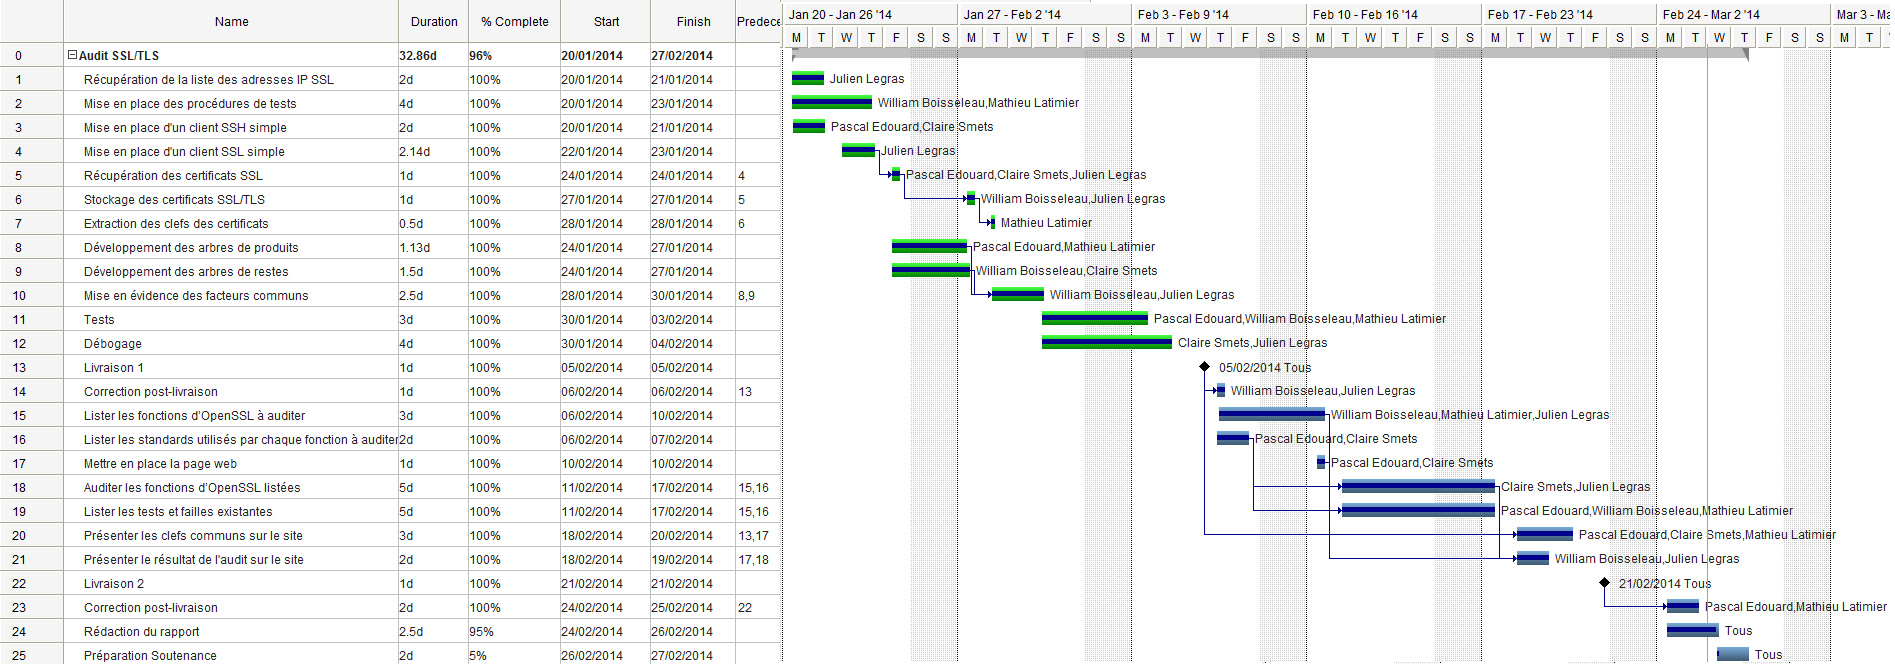
\includegraphics[scale=0.28]{images/projet_gantter.png}
\end{center}
\caption{Gantter}
\label{gantter}
\end{figure}

De plus, le diagramme du Gantter est plus esthétique que notre précédent diagramme, ce qui nous permettait de retrouver plus facilement nos informations.

\subsection{LaTeX et BibTeX}

Latex est un langage de structuration de documents créé en 1983 par Leslie Lamport. Il utilise des macro-commandes qui seront interprétés par le processeur de texte TeX.\\
BibTeX est un logiciel de gestion de références bibliographiques qui va nous servir à gérer et traiter notre base bibliographique à travers nos documents Latex.\\

Nous avons choisi de réalisé l'ensemble de nos documents (comptes-rendus, rapports, livrables) sous LaTeX pour qu'ils soient homogènes (nous partions sur la même base), réutilisables et modulaires (découpage sous forme de briques). Les éditeurs/compilateurs de LaTeX sont nombreux, nous avons optés pour deux d'entres eux : Gummi et TexMaker.

\section{Ressources de tests}

Pour nos tests nous avons eu besoin de quelques outils que nous détaillerons ci-dessous.

\subsection{Netkit}

Netkit est un environnement permettant de configurer et de tester un réseau virtuel rapidement et sans grandes ressources.\\
Lors des procédures de tests de la première partie, nous voulions générer un petit réseau comportant toutes les configurations possibles rencontrables lors du scannage, de la récupération de certificats et de la post-récupération (extraction de données, gestion des doublons, liens symboliques, etc...).\\
Nous avons donc décidé de réaliser ce petit réseau à l'aide de cet outil.

\subsection{Pencil}

Pencil \cite{pencil} est un logiciel de création de maquettes typographiques libre et gratuit développé par Evolution Solutions.
Nous nous sommes servi de ce logiciel afin de réaliser les maquettes des pages web attendues pour chacune des trois parties.\\
Le rendu final n'est pas exactement celui des maquettes car nous avons également utilisé plusieurs frameworks pour améliorer la qualité graphique (i.e. HighCharts, BootStraps), mais le contenu et la disposition est sensiblement la même.
Ces tests nous ont permis de partir sur une base commune.

\section{Ressources techniques}

Pour ce qui est du développement de scripts, de la gestion du site web avec base de données, et de la mise en place du navigateur sécurisé de la troisième partie, nous avons utilisé les machines de l'université et nos ordinateurs portables. Mais pour les parties plus délicates comme, le scannage de ports Internet, la récupération de certificats, ou la factorisation des moduli pour la première partie nous avions des ressources techniques plus importantes.

\paragraph{Connexion internet : } Pour la première partie, nous avions besoin d'une bonne connexion internet pour le scannage, ainsi que pour la récupération des certificats. Il fallait prendre certaines précautions afin de ne pas congestionner le réseau, et éviter également que le proxy ne dérange le déroulement des scripts. Par conséquent, nous avons lancer les scans importants les vendredi soirs, et en utilisant la prise ethernet extérieur.

\paragraph{Serveur de calcul de l'Université :} Ce serveur nous a permis de factoriser les moduli lors du deuxième scan (plus de 500.000 certificats), et de gagner du temps sur l'avancement de notre projet.

\section{Choix des langages de développement}

\subsection{Langage C et librairie GnuMP}

Nous avons décidé avant de débuter le projet de faire une étude en benchmark-test \cite{chooseprogram2013} \cite{marceau2009program} \cite{udemypng} (test de performance CPU, RAM, taille de code), sans oublier deux principes fondamentaux qui sont la gestion des grands entiers et les préférences de chacun (degré de compétence, aisance).\\
Les codes sont basés sur l'utilisation combinée de structures et d'algorithmes complexes (sur arbres, ensembles, anneaux, etc...).\\

Plusieurs langages ont étés testés parmis lesquels :
\begin{itemize}
\item C;
\item C++;
\item Java;
\item Perl;
\item Python;
\item Ruby;\\
\end{itemize}

Nous avons au final décidé d'utiliser le langage C avec la librairie GnuMP \cite{gmplib} pour la gestion des grands entiers, et le compilateur CMAKE.
Le langage C est l'un des plus rapide en temps d'exécution, il est également l'un de ceux qui consomme le moins de mémoire. Il est également très performant sur la gestion des grands entiers.\\
Le python et le C++ étés également de très bon choix, mais les développeurs ont une meilleure maitrise du C.

\subsection{Langages de scripts : Bash et Perl}

Nous avons opté également pour du développement de scripts pour des algorithmes peu complexes nécessitant plusieurs appels systèmes, surtout pour les commandes OpenSSL (extraction de moduli dans un certificat, connexion au serveur, récupération de champs dans un ensemble X509).\\
L'avantage des scripts est qu'ils sont facilement modifiables. On pouvait donc les réarranger pour les réutiliser à d'autres fins.

\subsection{IDE : Eclipse pour C}

Eclipse est un environnement de développement et gestionnaire de projets pouvant supporter plusieurs langages de développement comme le Java, l'Android, le C, le C++, etc...\\
Nous avons utilisé cet éditeur afin de mieux lire le code d'OpenSSL et d'identifier les failles à l'aide des différents commits de l'équipe OpenSSL. Nous l'avons également utilisé pour la troisième partie du projet.

\section{IHM}

\subsection{Site Web}

Nous avons établit un site web local afin de regrouper tout nos résultats sur une interface que nous pourrons offrir au client. Les trois parties sont certes indépendantes, mais elles se complètent parfaitement afin de mieux comprendre la sécurité actuelle de l'Internet, des protocoles SSL/TLS et du logiciel de génération de clés cryptographiques le plus répandu : OpenSSL.\\
L'ensemble du site web repose sur le framework \textbf{BootStrap}.\\

Sur le premier onglet nous avons réaliser des études statistiques sur les certificats SSL récupérés (certificats contenant des facteurs communs à d'autres certificats, regroupement par \textit{issuer}, recherche utilisateur, tri par taille de clés, etc...).\\
Les certificats sont stockés en base \textbf{MySQL}, et les graphiques sont générés via le framework \textbf{HighCharts}.\\

Sur le second onglet nous listons quelques primitives cryptographiques d'OpenSSL à auditer. Nous avons intégré deux modes un en écriture et un en lecture seule, et chaque élément de cette page est enregistré dans notre base de données.\\

Enfin, sur le dernier onglet, nous étudions la sécurité du navigateur client en affichant les algorithmes de chiffrement, les algorithmes de signatures, les méthodes de compressions, les versions de protocoles, les courbes elliptiques et les tickets de sessions. Un code couleur est également défini afin d'identifier les \textit{ciphersuites} faibles (Jaune), critiques (Rouge) et fortes (Verte).

\subsection{Doxygen}

Doxygen est un générateur de documentation sous licence libre capable de produire une documentation logicielle à partir du code source d'un programme. Il supporte entre autres le langage C qui est le langage de développement utilisé par OpenSSL. Nous avons décidé de rediriger le code source d'OpenSSL sous Doxygen pour faciliter sa compréhension, et pouvoir analyser plus facilement l'arborescence de la fonction.\\
La fonction de recherche de code de Doxygen nous a également fait gagner du temps, notamment sur le choix des primitives cryptographiques à étudier et l'identification de vulnérabilités.\\

\section{Gestion des risques}

Durant ces six semaines, nous avons été confrontés à deux risques que nous avions listés dans le document d'analyse des risques.
\begin{itemize}
\item Nous avons eu régulièrement des absences occasionnelles, en grande partie à cause des entretiens pour nos stages, mais aussi pour des problèmes d'administration, de cours, maladies, empêchements.
\item Nous n'avons pas pu récupérer les adresses IP des serveurs SSH, le scan de port SSH étant interdit nous avons reçu une plainte d'Amazon, et nous avons décidé avec l'accord du client d'abandonner cette partie.\\
\end{itemize}

Pour le premier point, nous avons bien suivi le plan d'action, en partant sur une base de travail de 8h par jour, et en rattrapant le retard accumulé si possible en semaine ou le samedi. Notre bonne organisation nous a permis de ne pas accumuler de retard, et de pouvoir prendre rapidement la tâche d'un autre en cas d'absence prolongée.\\

Aucun autre risque identifié n'est survenu durant le projet.
